\section{Mesh Network}\label{sec:mesh-network}

In a centralised environment each client communicates with a central server. Therefore clients do not have to know other clients.
Nodes in a decentralised network do not have a central counterpart. Thus a node has to discover other nodes and establish connections to them.

One common standard to achieve this is \gls{ip} multicast. The multicast concept operates on OSI-Layer 3 and is based on groups. Anyone can create a group with a unique address where others can receive packets from and send packets to \cite[pp. 484-485]{tanenbaum_wetherall_2011}. Based on ping messages the liveliness of group members is periodically checked. When a packet is addressed to a group, the router has to duplicate packets and broadcast them to all nodes. 
The use cases for multicast are unlimited: group chats, conference calls or tv broadcasting.
However, due to technical limitations like scaling issues and limited address space, it has not proven to be successful yet \cite{multicast}.
As multicast is not widely deployed, a decentralised network has to be constructed manually \cite[\S1]{multicast-problems}.

An overlay network where nodes are connected with each other in an autonomous manner is called Mesh Network. The easiest approach is to connect all the nodes with each other, which would result in a fully connected mesh network. However, with a growing number of participants this approach becomes unfeasible, because each node can only handle a limited amount of connections.

Due to this limitation a node can only connect to a subset of the total available nodes. To reach nodes without a direct connection it has to make use of other nodes as forwarders. Therefore packets have to be routed through the network by a routing protocol.

\subsection{Broadcasting Routing Protocols}
In the easiest scenario of a decentralised network a node is broadcasting a packet to all other nodes in the network. For this scenario the node does not need to know about the presence of other nodes besides the nodes it is directly connected with.

\paragraph{Flooding}\label{flooding}
A node sends a packet to all directly connected nodes where the packet is then again forwarded to all their direct nodes. Eventually, all the nodes in the network will receive the packet. 

The process of forwarding a packet to all direct connected nodes is one of simplest message routing algorithms and called \textit{Flooding} \cite[p. 368]{tanenbaum_wetherall_2011}

To prevent infinite hopping, the broadcast packet has to be dropped at some point. One option to achieve this is, is to set a \gls{ttl} on the packet. Each hop that is receiving a packet is decreasing the \gls{ttl} by one. As long as the \gls{ttl} is greater than zero the packet is forwarded, otherwise it is dropped. One issue that arises by a \gls{ttl} is, that it may not reach all the nodes in the network because it is discarded before.

When it is reaching all nodes has priority, another option is to set a sequence number on the packet.
A node, that receives a packet with a sequence number, can check whether it has received a packet with that sequence already. When the sequence number is new, it is stored and the packet is forwarded. When the sequence number has been seen already the packet is dropped silently.

\begin{figure}
\centering
\includegraphics[width=1\textwidth]{graphics/flooding-with-sequence.pdf}
\caption{Flooding a packet with a sequence number}
\label{fig:flooding}
\end{figure}

\cref{fig:flooding} shows the flow of a packet that has been dispatched by \textit{A} with the sequence number \textit{\#1}. \textit{A} is increasing its own sequence number for the next packet. \textit{B} and \textit{C} receive the packet and as the sequence number is unknown they forward the message to their connected nodes (\textit{B}$\rightarrow$\textit{C}\&\textit{D},  \textit{C}$\rightarrow$\textit{B}\&\textit{D}). \textit{B} and \textit{C} receive a packet with a sequence number both have already seen, so the message is dropped. The sequence number prevents an infinite back and forth hopping that would otherwise clog the network.

The Flooding mechanism is tremendously effective win terms of reaching all nodes in the network. In fact, it will find the shortest path to all nodes, due to the fact that all paths are tried.
However, it also generates a lot of overhead traffic. As seen in \vref{fig:flooding}, \textit{B} $\leftrightarrow$ ︎\textit{C} and \textit{D} $\leftrightarrow$ \textit{E} are sending the packets back to each other as they do not know, that the counterpart has seen the packet already. The packet is dropped, yet it is an unnecessary transmission.

\paragraph{Gossiping}\label{gossiping}
\largepage
Gossip Protocols take human nature and epidemics as a role model how to spread information inside the network \cite[\S1]{Jelasity2011}. 
In a nutshell it works similar to \textit{Flooding} but instead of forwarding to all directly connected nodes, only a subset is selected. Different selection strategies exist, like random selection or selection based on a heuristic. 
\say{Infected} nodes continue the process by selecting their best nodes. This is almost as effective as \textit{Flooding} as \citet{riviere_voulgaris_2011} phrase it \say{Making a random selection out of a random subset of all nodes is equivalent to making a random selection out of \textit{all} nodes.}
However, as the there is a node selection, it is not as efficient as \textit{Flooding} in terms of time until the packet has reached all otehr nodes.

\citet{Jelasity2011} describes two models of \textit{Gossip} SI and SIR:

\begin{itemize}
\item susceptible (S): The node does not know about the update
\item infected (I): The node knows the update and is actively spreading it
\item removed (R): The node has seen the update, but is not participating in the spreading process (in epidemiology, this corresponds to death or immunity)
\end{itemize}
\cite[\S1.2.2]{Jelasity2011}

Those are the three states a node can have when a \textit{Gossip} packet is spread through the network.

SI:
In the SI-Model a node is in \textit{\textbf{S}usceptible} state until it receives a \textit{Gossip} packet from another node. On receive it switches into the \textit{\textbf{I}nfected} state and starts spreading it in a fixed interval to selected nodes. This is the \textit{push}-variant of the SI-Model. There is also a \textit{pull}-variant where a node acts passively and only asks neighbour nodes whether they have a \textit{Gossip} packet. A third variant is the \textit{push-pull}-variant where nodes are actively spreading the packet as soon as they switch into the \textit{\textbf{I}nfected} state, but also ask neighbours whether they have a \textit{Gossip} packet.

\begin{Listing}
\begin{lstlisting}[multicols=2,basicstyle=\tiny,basicstyle=\footnotesize\ttfamily,xleftmargin=3em]
loop
  wait()
  p <- random peer
  if push and in state I then
    send update to p
  end if
  if pull then
    send update-request to p
  end if
end loop

procedure ONFEEDBACK(m)
  switch to state R with prob. 1/k |\label{line:SIROnFeedback}|
end procedure
procedure ONUPDATE(m)
  if in state I or R then
    send feedback to m.sender |\label{line:SIRfeedback}|
  else
    store m.update // now in state I
  end if
end procedure

procedure ONUPDATEREQUEST(m)
  if in state I then
    send update to m.sender
  end if
end procedure
\end{lstlisting}
\caption{SIR from \cite[\S1.2.2.2]{Jelasity2011}}
\label{lst:SIRAlgo}
\end{Listing}

SIR:
SIR extends SI with a third state: \textit{\textbf{R}emoved}. While the SI-Model will never terminate spreading the \textit{Gossip} packet, thus producing a lot of unnecessary traffic, SIR terminates the spreading, as soon as the node switches into the \textit{Removed} state.

\Cref{lst:SIRAlgo} shows the basic functionality of SIR. 
When the node receives a \textit{Gossip} packet it has already seen, it sends feedback to the sender of the packet (line \ref{line:SIRfeedback})
On feedback, a node that has send a \textit{Gossip} packet, can switch to state \textit{Removed} (line \ref{line:SIROnFeedback}). In the described algorithm this happens with a probability of 1/\textit{k}, \say{where the natural interpretation of parameter k is the average number of times a node sends the update to a peer that turns out to already have the update}\cite[\S1.2.2.2]{Jelasity2011}. When the node is in state \textit{Removed} it will not send any updates to other nodes anymore.

\subsection{Node Discovery}
The previous described routing protocols rely on the assumption that a node does not need to know the whole network. They only need to know directly connected nodes, in order to forward packets.
For many scenarios the only knowledge of direct nodes is not enough. In fact, in many scenarios a bigger picture of the network is needed or at least the knowledge about the presence of another node. This involves node discovery. However, a node that has discovered other node does not need a connection to them, it only needs to know that the node is somehow reachable.
Node discovery, path discovery and maintenance are tasks that \textit{Reactive Routing} and \textit{Proactive Routing} protocols are dealing with.

\subsection{Reactive Routing}
Reactive protocols act passively, meaning that they are not actively looking for nodes but only when a packet has to be forwarded to an unknown node.
When a packet is received by a node that is not meant to be the receiver, the node has to forward the packet. In case it does not have any routing information, it has to acquire them. 
To acquire routing information it can make use of \textit{Flooding} (\cref{flooding}) and flood a route request to its directly connected nodes. \say{These neighbours forward the route request packet to their neighbours and this process goes on until either the target node or an intermediate node with a valid route to target node is located. Each node receiving a particular route request packet broadcasts it only once to its neighbours, and it discards the subsequent receptions of the same route request packet, to minimise routing overhead} as described by \citet[\S1.3]{Mukhija_Arun}. 
Reactive Protocols are for example AODV, DSR, TORA which are compared by \citet{kalwar_2010}

\subsection{Proactive Routing}
In comparison to the passively acting \textit{Reactive protocols} the proactive, are actively gathering information about the network, by periodically sending \textit{Ping}-Packets. Each node is maintaining a routing table. When it receives a Ping-Packet from an unknown node the node is added to the routing table with the last hop neighbour as originator. The node is now able to reach the added node via the originator. 
There are different approaches how Ping packets are propagated through the network. Most of them also rely on \textit{flooding} or \textit{gossiping}.
A expiration mechanism has clean up stalled nodes, where no \textit{Ping}-Packet has been received for a defined number. Otherwise, a node would stay in the table for ever, even though it has lost its connection to the network a long time ago.

\subsection{OSLR}\label{sec:mesh-oslr}
\gls{olsr} is a proactive routing control, which is optimising the amount of Ping-Packets needed to discover other nodes in the network. OSLR calls those Ping-Packets \textit{HELLO}-Packets.
A node that is directly connected to another node is seen as a \textit{1-Hop Neighbour}. \textit{1-Hop Neighbours} are exchanging continuously \textit{HELLO}-Packets where they also include all known \textit{1-Hop Neighbours}.

On receive, the node is adding all neighbours that are included in the \textit{HELLO}-Packet as \textit{2-Hop-Neighbours} into their neighbour table. Excluding all direct nodes from \textit{2-Hop-Neighbours}, results in the \textit{Strict-2-Hop-Neighbours}.
Based on the list of known nodes it is now selecting \glspl{mpr}. \Glspl{mpr} are \say{selected such that it covers (in terms of radio range) all symmetric strict 2-hop nodes.}\cite[\S1.4]{rfc-oslr}. A node that has selected a \gls{mpr} is a \textit{MPR-Selector}. Nodes are \say{upgraded} to \gls{mpr} by a \textit{HELLO}-Packet, which can also include a list of selected \glspl{mpr}.

\Glspl{mpr} are disseminating \gls{tc} packets to all their nodes with the list of their \textit{MPR-Selectors} and their sequence number, that represents the sequence of the \gls{mpr} nomination.
When a node receives the \gls{tc} packet, it is setting up a topology table with the last-hop neighbour, the selected \gls{mpr} and the sequence number of the selected \gls{mpr}.

Each node is maintaining also a \textit{Routing table} which aggregates the \textit{Neighbour table} and the \textit{Topology table} into one. Entries of the \textit{Routing table} are all the nodes that can be addressed as long as they have not left the network. 

Based on the \textit{Routing table} a node tries to find the optimal path to each entry. \citet[\S4.4]{jacquet_muhlethaler_clausen_laouiti_qayyum_viennot} describe in detail how the routing table is calculated.

\subsection{B.A.T.M.A.N}\label{sec:batman}
Another approach is the \textit{B.A.T.M.A.N} Protocol which stands for \textbf{B}etter \textbf{A}pproach \textbf{T}o \textbf{M}obile \textbf{A}d hoc \textbf{N}etworking and is developed by the Freifunk Community.

It makes use of \textit{gossiping}(cf. \vref{gossiping}) to disseminate \glspl{ogm} through the network. Each node is sending a \gls{ogm} to their direct neighbour. \say{These neighbours are re-broadcasting the OGMs according to specific rules to inform their neighbours about the existence of the original initiator of this message and so on and so forth. Thus the network is flooded with originator messages.} as described in the concept of \citet{batman}.

Unlike other protocols, where the packet is not sent back to the sender, B.A.T.M.A.N is also answering to the sender by sending the packet back. Those packets are called \textit{Echo} packets. By doing so it each node is calculating the \gls{tq} to each direct neighbour by counting the total amount of \gls{ogm} packets received from that node—\gls{rq} and the amount of \textit{Echo}-\gls{ogm} packets received—\gls{eq}. 
The packets are counted by using a sliding window \cite[\S3.4]{tanenbaum_wetherall_2011} with a fixed size. \cref{fig:sliding-window} shows a sample sliding window with size 2. 

\begin{figure}
\centering
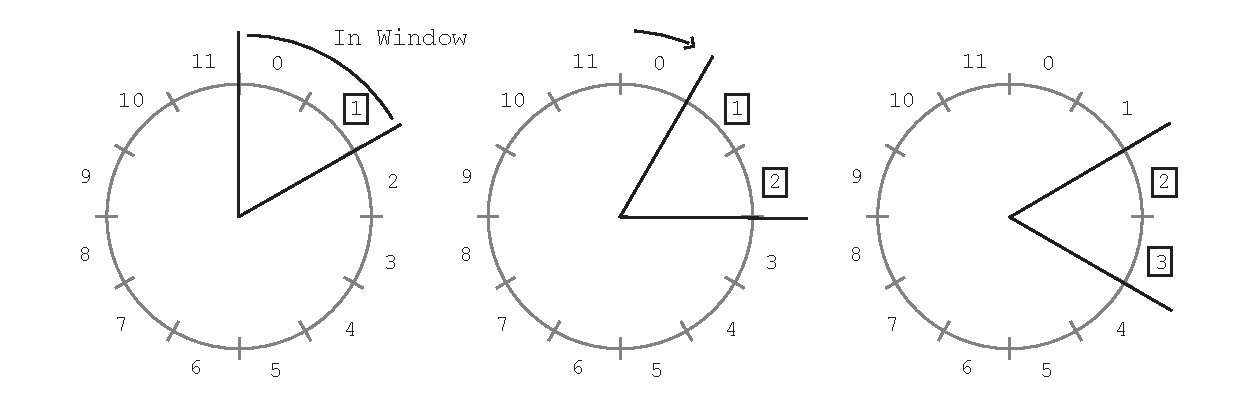
\includegraphics[width=1\textwidth]{graphics/sliding-window.pdf}
\caption{A sample sliding window}
\label{fig:sliding-window}
\end{figure}

When an \gls{ogm} is received, a node checks whether it is one that it has send, thus an \textit{Echo} packet. When it is an \textit{Echo} packet, it checks the outgoing sliding window whether the sequence number is in-window. If it is, the sequence number is added to the sliding window. By counting all values of the sliding window the node obtains the \gls{eq}. 
Otherwise, the node checks the incoming sliding window. When the sequence number is out of window it adds the sequence, slides the window to the new sequence number and drops all sequences out of window. This results in the \gls{rq}.

\say{With both values, it is possible to determine, whether the link is a bidirectional one and to create a metric to compare different links.}\cite[\S2.3.3]{tobias_hardes}. The value is determined by dividing the \gls{eq} through \gls{tq}.

\begin{equation}
\label{eq:transmit_quality}
\gls{tq} = \frac{\gls{eq}}{\gls{rq}}
\end{equation}

A \gls{tq} value of $\ 1 $ indicates that the outgoing connection to the other node is as good as the incoming. A value less than $\ 1 $ indicates package loss.

\glspl{ogm} are initialised with the next sequence number of the outgoing sliding-window, an initial \gls{tq} and an initial \gls{ttl} (initial \gls{tq} and \gls{ttl} are both fixed values). On receive of an \gls{ogm}, a node is checking whether the sequence number is out of the receive sliding-window. In case it is not, the node has already received the packet from another node. Thus the \gls{ogm} is dropped. For a first-time seen sequence number the node is processing the \gls{tq} value of the \gls{ogm}. It is multiplying the calculated \gls{tq} to the last sender of the packet with the current \gls{tq} value of the packet. Also a hop penalty is subtracted, in order to punish routes with many hops because each hop endangers a successful transmission. The \gls{tq} and the \gls{ttl} of the \gls{ogm} are limiting the traffic impact. Without the limitation, the whole network would eventually get \glspl{ogm} of any other node and the traffic impact would be too high.

\begin{equation}
\label{eq:ogm_quality}
new\_ogm\_tq = ogm\_tq * last\_hop\_tq * hop\_penalty
\end{equation}

When the resulting \gls{tq} is greater than zero, the sender of the \gls{ogm} is added into the routing table with the \gls{tq} value of the \gls{ogm}, unless the originator is already a direct neighbour. The \gls{tq} of the Routing-Table helps a node to determine which is the best router for a message.

\begin{figure}
\centering
\includegraphics[width=0.7\textwidth]{graphics/batman.pdf}
\caption{Sample graph}
\label{fig:sample-graph-with-tq}
\end{figure}

\vref{fig:sample-graph-with-tq} shows a sample graph with nodes that have calculated the \gls{tq} to their direct neighbours. The \gls{tq} for the multi–hop neighbours has to be calculated by exchanging \gls{ogm}.

\vref{tbl:sample-tq-table} shows the deviated routing table of \textit{Node A}

\begin{table}[htb!]
  \centering
  \begin{tabu} to \textwidth {X[c]X[c]X[c]}
		\toprule
    		\textbf{Originator} & \textbf{Next–Hop} & \textbf{TQ} \\
		\midrule
		B & B & 80.0 \\
		B & C & 17.5\\
		C & C & 60.0 \\
		C & B & 23.3 \\
		D & B & 43.2\\
		D & C & 32.4\\
		E & B & 15.5 \\
		E & C & 37.8 \\
		\bottomrule 
	\end{tabu}
\caption{Sample routing table for \textit{Node A} based on \cref{fig:sample-graph-with-tq}}
\label{tbl:sample-tq-table}
\end{table}

\paragraph{Example TQ for Node E}
For the calculation of the the \gls{tq} value an initial \gls{ogm}-\gls{tq} of 100 and a \textit{hop penalty} of 0.9 is given.
The \gls{tq} of \textit{Node E} arises from the path taken by the \gls{ogm}.
When \textit{Node E} dispatches its \gls{ogm} it is taking the path E$\rightarrow$C$\rightarrow$A and E$\rightarrow$D$\rightarrow$B$\rightarrow$A. \vref{eq:tq_example} shows how the \gls{tq} is calculated.

\begin{equation}
\label{eq:tq_example}
\begin{aligned}
\gls{tq} _{next-hop-C} = & \overrightarrow{EC} (100 * 0.7 * 0.9) * \overrightarrow{CA} (0.6) = \textbf{37.8} \\
\gls{tq} _{next-hop-B} = & \overrightarrow{ED} (100 * 0.4 * 0.9) * \overrightarrow{DB} (0.6 * 0.9) * \overrightarrow{BA} (0.8) = \textbf{15.5}
\end{aligned}
\end{equation}

By sorting the table by \gls{tq} \textit{Node A} would send its message via \textit{Node B} because the \gls{tq} is better than the one of \textit{Node C}.
